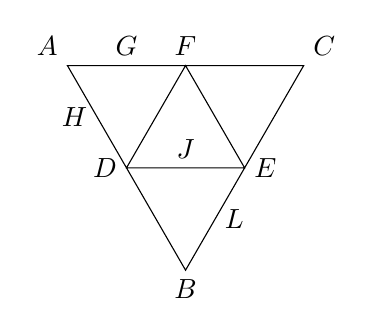
\begin{tikzpicture}[scale=1.5]
\coordinate (A) at (0,1.732); \coordinate (B) at (1,0); \coordinate (C) at (2,1.732); \coordinate (D) at (.5,.866); \coordinate (E) at (1.5,.866); \coordinate (F) at (1,1.732); \coordinate (G) at (.5,1.732); \coordinate (H) at (.25,1.299); \coordinate (I) at (1.25,.433); \coordinate (J) at (1,.866);
\draw (A)--(B)--(C)--cycle (D)--(E)--(F)--cycle;
\node[above left] at (A) {$A$}; \node[below] at (B) {$B$}; \node[above right] at (C) {$C$}; \node[left] at (D) {$D$}; \node[right] at (E) {$E$}; \node[above] at (F) {$F$}; \node[above] at (G) {$G$}; \node[left] at (H) {$H$}; \node[right] at (I) {$L$}; \node[above] at (J) {$J$};
\end{tikzpicture}
